\chapter{System Description}


\section{First Section}


\subsection{Fist Subsection}


\subsection{Another Subsection}

\begin{table}
    \centering
    \ra{1.1}
    \begin{tabular}{lp{0.4\linewidth}}
    \toprule
    \emph{Quant.} & \emph{Ingredient}\\
    \midrule
		200g &Wei{\ss}mehl\\
		1/4  &Packung Frischhefe\\
		4EL  &lauwarme Milch\\
		4EL  &�l\\
		1TL  &Zucker\\
		1TL  &Salz\\
		&lauwarmes Wasser\\
    \bottomrule
    \end{tabular}
    \caption[Flammkuchenteig]{Flammkuchenteig. The ingredients have to be carefully chosen.\label{tab:mytable}}
\end{table}



\begin{figure}
    \centering
    \setlength{\tabcolsep}{0.0130\linewidth}
    \begin{tabular}{@{}cc@{}}
    
\includegraphics[width=0.487\linewidth]{figures/TiltBrush_StarryNight}&
    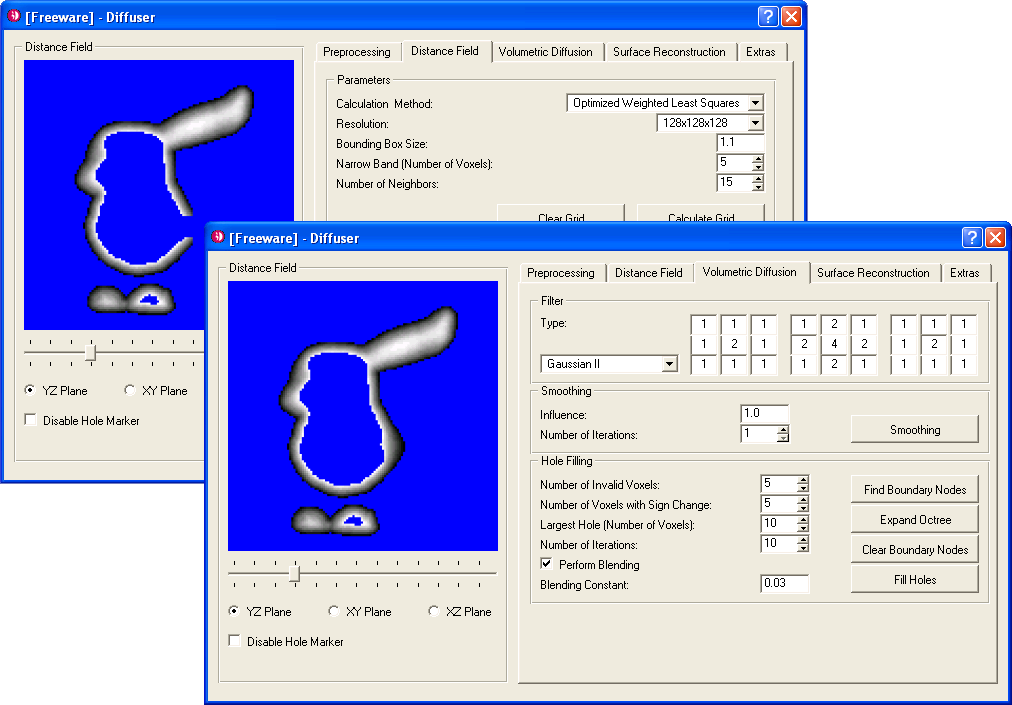
\includegraphics[width=0.487\linewidth]{figures/voldiff_ui}\\
    (a)&(b)\\
    \end{tabular}
    \caption[Volumetric diffusion]{Volumetric diffusion.
    	  \textup{(a)} Slices of the distance volume reveal the narrow band.
			  \textup{(b)} The user interface of the automatic hole filling
        tool allows to fine-tune the algorithm.
        The volumetric representation can be previewed before
        surface reconstruction.%
      \label{fig:voldiff}}
\end{figure}





\section{Second Section}

